\newpage

\section{Actividad 3: Curva Característica}

 \subsection{Objetivo:}
Obtener las diferentes curvas características del transistor NPN utilizando dos
fuentes variables que permitirán obtener las diferentes corrientes y tensiones del transistor.

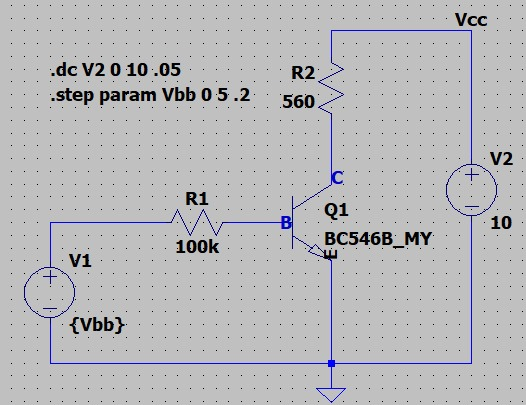
\includegraphics[width=7cm]{./imagenes/Circuito3.jpg}

\subsection{Materiales usados:}
\begin{itemize}
    \item Transistor BC546/7/8/9.
    \item Resistores $R_B = \SI{100}{\kilo\ohm}$, $R_c = \SI{560}{\ohm}$.
    \item Dos fuentes variables de 0V hasta (al menos) 10V.
\end{itemize}


\subsection{Procedimiento}

El procedimiento para la obtención de las curvas es repetitivo. Se realizará un barrido de la VCC por cada incremento de VBB (en función de $I_B$). Por cada cambio de $I_B$ se debe llevar a 0V la fuente VCC.

\begin{itemize}
  \item Con $V_{CC}=0$V e $I_B=0$A, realice un barrido de la tensión $V_{CC}$ y trate de obtener los valores que especifica la tabla 2 (primera columna). Registre el valor de $I_C$ y $V_{CE}$. Analice con profundidad lo que espera medir y debe apoyarse con la simulación.
  \item Vuelva a configurar $V_{CC}=0$V e intente lograr un incremento de 10$\mu$A para $I_B$. \textbf{Importante:} Si no tiene un instrumento con resolución de $\mu$A se puede obtener el valor de la corriente $I_B$ utilizando el método indirecto mediante la tensión que cae en el resistor $R_B$ y su valor óhmico. Es la principal razón por lo que se elige un valor de 100k$\Omega$ (su valor significativo de tensión será similar a la corriente).
  \item Repita el paso anterior para otro pequeño incremento de 5$\mu$A y tome las mediciones. Recuerde que la tabla 2 es un ejemplo, debe ajustar la misma a sus condiciones de ensayo y en base a las conclusiones que haya llegado mediante la simulación. Es decir, tenga presente qué pasaría si $I_B=0$A, o si es posible lograr $V_{CE}=10$V. Es importante que sea criterioso, la propuesta es analizar el comportamiento del transistor y con los conocimientos que dispone, es posible que pueda dar respuestas a estos puntos.
  \item Cada variación de corriente $I_B$ es una curva medida, se solicita que se obtenga mínimo 5 curvas.
\end{itemize}

\subsection{Tablas de medición}

\begin{table}[ht]
\resizebox{\columnwidth}{!}{%
\begin{tabular}{|
>{\columncolor[HTML]{FFCC67}}l |ll|ll|}
\hline
\cellcolor[HTML]{FFCC67} &
  \multicolumn{2}{l|}{\cellcolor[HTML]{96FFFB}\begin{tabular}[c]{@{}l@{}}$I_B=10 \mu A$\\ $V_{BB} = 1,6 V$\end{tabular}} &
  \multicolumn{2}{l|}{\cellcolor[HTML]{96FFFB}\begin{tabular}[c]{@{}l@{}}$I_B=15 \mu A$\\ $V_{BB} = 2,2V$\end{tabular}} \\ \cline{2-5} 
\multirow{-2}{*}{\cellcolor[HTML]{FFCC67}\begin{tabular}[c]{@{}l@{}}$V_{CC}$\\ {[}V{]}\end{tabular}} &
  \multicolumn{1}{l|}{\cellcolor[HTML]{67FD9A}$I_C$} &
  \cellcolor[HTML]{67FD9A}$V_{CE}$ &
  \multicolumn{1}{l|}{\cellcolor[HTML]{67FD9A}$I_C$} &
  \cellcolor[HTML]{67FD9A}$V_{CE}$ \\ \hline
0,25 & \multicolumn{1}{l|}{$339,95 \mu A$} & $59,65 mV$  & \multicolumn{1}{l|}{$358,29 \mu A$} & $49,37 mV$  \\ \hline
0,5  & \multicolumn{1}{l|}{$743,75 \mu A$} & $83,49 mV$  & \multicolumn{1}{l|}{$768,11 \mu A$} & $69,85 mV$  \\ \hline
1    & \multicolumn{1}{l|}{$1,57 mA$}      & $116 mV$    & \multicolumn{1}{l|}{$1,61 mA$}      & $95,94 mV$  \\ \hline
2    & \multicolumn{1}{l|}{$2,95 mA$}      & $347,25 mV$ & \multicolumn{1}{l|}{$3,32 mA$}      & $138,53 mV$ \\ \hline
5    & \multicolumn{1}{l|}{$3 mA$}         & $3, 26 V$   & \multicolumn{1}{l|}{$4,88 mA$}      & $2,26 V$    \\ \hline
10   & \multicolumn{1}{l|}{$3,34 mA$}      & $8,12 V$    & \multicolumn{1}{l|}{$5,27 mA$}      & $7,04 V$    \\ \hline
\end{tabular}%
}
\end{table}


\begin{table}[ht]
\resizebox{\columnwidth}{!}{%
\begin{tabular}{|
>{\columncolor[HTML]{FFCC67}}l |ll|ll|}
\hline
\cellcolor[HTML]{FFCC67} &
  \multicolumn{2}{l|}{\cellcolor[HTML]{96FFFB}\begin{tabular}[c]{@{}l@{}}$I_B=20 \mu A$\\ $V_{BB} = 2,6V$\end{tabular}} &
  \multicolumn{2}{l|}{\cellcolor[HTML]{96FFFB}\begin{tabular}[c]{@{}l@{}}$I_B=25 \mu A$\\ $V_{BB} = 3,2V$\end{tabular}} \\ \cline{2-5} 
\multirow{-2}{*}{\cellcolor[HTML]{FFCC67}\begin{tabular}[c]{@{}l@{}}$V_{CC}$\\ {[}V{]}\end{tabular}} &
  \multicolumn{1}{l|}{\cellcolor[HTML]{67FD9A}$I_C$} &
  \cellcolor[HTML]{67FD9A}$V_{CE}$ &
  \multicolumn{1}{l|}{\cellcolor[HTML]{67FD9A}$I_C$} &
  \cellcolor[HTML]{67FD9A}$V_{CE}$ \\ \hline
0,25 & \multicolumn{1}{l|}{$366,27 \mu A$} & $44,9 mV$   & \multicolumn{1}{l|}{$375,06 \mu A$} & $39,97 mV$  \\ \hline
0,5  & \multicolumn{1}{l|}{$778,46 \mu A$} & $64,06 mV$  & \multicolumn{1}{l|}{$789,82 \mu A$} & $57,7 mV$   \\ \hline
1    & \multicolumn{1}{l|}{$1,62 mA$}      & $88,19 mV$  & \multicolumn{1}{l|}{$1,64 mA$}      & $80 mV$     \\ \hline
2    & \multicolumn{1}{l|}{$3,35 mA$}      & $123,46 mV$ & \multicolumn{1}{l|}{$3,37 mA$}      & $110,52 mV$ \\ \hline
5    & \multicolumn{1}{l|}{$5,98 mA$}      & $1,64 V$    & \multicolumn{1}{l|}{$7,53 mA$}      & $783,2 mV$  \\ \hline
10   & \multicolumn{1}{l|}{$6,46 mA$}      & $6,37 V$    & \multicolumn{1}{l|}{$8,13 mA$}      & $5,44 V$    \\ \hline
\end{tabular}%
}
\end{table}

\subsection{Gráficos}

En base a los datos obtenidos en las tablas anteriores, podemos graficar las curvas características del transistor BC548.

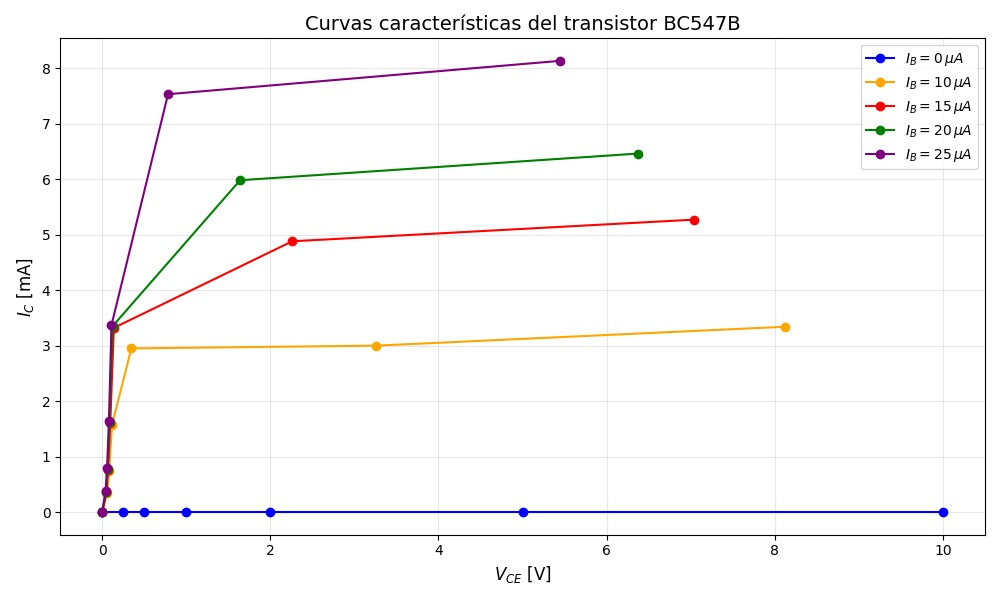
\includegraphics[width=8cm]{./imagenes/Grafico3.jpg}

\subsection{Conclusiones}

Como se observa en las tablas, despreciamos la parte de las mediciones para cuando ambas fuentes son 0, ya que los valores de $V_{CE}$ y de $I_C$ son irrelevantes en ese punto de operación, incluso algunos estan dados por la mala regulacion de voltaje de las fuentes, ya que es muy complicado llevarlas exactamente al 0.
